\documentclass[11pt,a4paper]{book}
\usepackage[brazilian]{babel}
\usepackage[utf8]{inputenc}
\usepackage[T1]{fontenc}
\usepackage[inline]{enumitem}
\usepackage{xcolor}
\usepackage{listings}
\usepackage{graphicx}
\usepackage{multicol}
\usepackage{amsmath}
\usepackage{amssymb}

\definecolor{mGreen}{rgb}{0,0.6,0}
\definecolor{mGray}{rgb}{0.5,0.5,0.5}
\definecolor{mPurple}{rgb}{0.58,0,0.82}
\definecolor{backgroundColour}{rgb}{0.95,0.95,0.92}

\lstdefinestyle{CStyle}{
    backgroundcolor=\color{backgroundColour},   
    commentstyle=\color{mGreen},
    keywordstyle=\textbf{\color{black}},
    numberstyle=\tiny\color{mGray},
    stringstyle=\color{mPurple},
    basicstyle=\footnotesize,
    breakatwhitespace=false,         
    breaklines=true,                 
    captionpos=b,                    
    keepspaces=true,                 
    numbers=left,                    
    numbersep=5pt,                  
    showspaces=false,                
    showstringspaces=false,
    showtabs=false,                  
    tabsize=2,
    frame=single,
    escapeinside={(*}{*)},
    language=C
}

\makeatletter
% This command ignores the optional argument for itemize and enumerate lists
\newcommand{\inlineitem}[1][]{%
\ifnum\enit@type=\tw@
    {\descriptionlabel{#1}}
  \hspace{\labelsep}
\else
  \ifnum\enit@type=\z@
       \refstepcounter{\@listctr}\fi
    \quad\@itemlabel\hspace{\labelsep}
\fi}
\makeatother

\newcommand{\onestaritem}{\refstepcounter{enumi}\item[$*$\theenumi.]}
\newcommand{\twostaritem}{\refstepcounter{enumi}\item[$**$\theenumi.]}
\DeclareMathOperator*{\maxi}{max}

\title{Lista 11: Fundamentos Estatísticos para Ciência dos Dados}
\author{Ricardo Pagoto Marinho}

\begin{document}
\maketitle
	\begin{enumerate}
		\item
		
		Fazendo a análise:
		
		\begin{lstlisting}
beetles <- read.table('BEETLES.DAT', col.names = c('
Measurement.Number', 'Species', 'transverse.groove.dist',
'elytra.length', 'second.antennal.joint.length',
'third.antennal.joint.length'))
library(dplyr)
beetle1 <- filter(beetles, Species == 1)[,3:6]
beetle2 <- filter(beetles, Species == 2)[,3:6]
n1 <- nrow(beetle1)
n2 <- nrow(beetle2)
beetle1.means <- apply(beetle1, 2, mean)
beetle2.means <- apply(beetle2, 2, mean)
w1 <- (n1 - 1) * var(beetle1)
w2 <- (n2 - 1) * var(beetle2)
sp1 <- 1 / (n1 + n2 - 2) * (w1 + w2)
a <- solve(sp1) %*% (beetle1.means - beetle2.means)
diag(sp1)^(1/2) * a
library(MASS)
beet.lda <- lda(Species ~ .-Measurement.Number, data = beetles)
beet.lda$scaling
beet.lda$scaling / a
plot(beet.lda)

		\end{lstlisting}
		
		\begin{figure}[h]
		\centering
		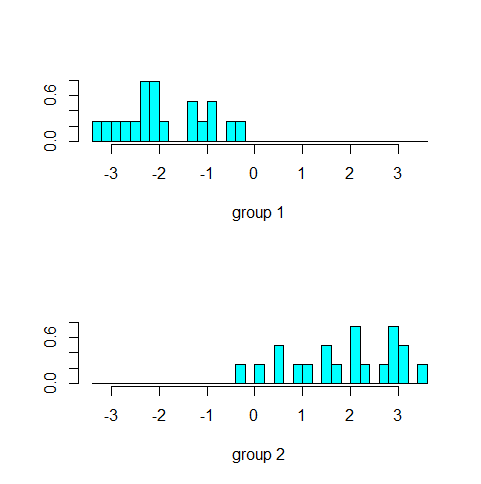
\includegraphics[height=6cm]{Rplot.png}
		\end{figure}
		\item
		\begin{itemize}
		
			\item
			
			Para o caso de $c(1|2)=c(2|1)$ e $\pi_1=\pi_2$, a comparação fica reduzida apenas à quantidade de indivíduos nas duas amostras, já que o que vai definir a região é qual função de densidade é a maior.
			
			\item 
			
			Para $\pi_1=0.001$, consequentemente $\pi_2=0.99$ e $c(1|2)=c(2|1)$, a função de classificação fica:
			
			\begin{eqnarray*}
				\frac{f_1(x)}{f_2(x)}>&\frac{\pi_2}{\pi_1}\\
				\frac{f_1(x)}{f_2(x)}>&\frac{0.99}{0.01}\\
				\frac{f_1(x)}{f_2(x)}>&99\\
				f_1(x)>&99f_2(x)
			\end{eqnarray*}
			
			Ou seja, $f_1(x)$ deve ser mais do que 99 vezes maior do que $f_2(x)$
			
			\item
			
			Neste caso, com $c(1|2)=\frac{c(2|1)}{10}$ e $\pi_1=0.001$ e $\pi_2=0.99$ temos: 
			
			\begin{eqnarray*}
				\frac{f_1(x)}{f_2(x)}>&\frac{c(1|2)}{c(2|1)}\frac{\pi_2}{\pi_1}\\
				\frac{f_1(x)}{f_2(x)}>&\frac{c(2|1)}{10}\frac{1}{c(2|1)}\frac{0.99}{0.01}\\
				\frac{f_1(x)}{f_2(x)}>&\frac{0.99}{0.1}\\
				\frac{f_1(x)}{f_2(x)}>&9.9\\
				f_1(x)>&9.9f_2(x)
			\end{eqnarray*}
			
			Ou seja, a regra do item anterior fica 10 vezes menor, já que aqui, $f_1(x)$ deve ser mais do que 9.9 vezes maior do que $f_2(x)$.
		\end{itemize}
		
		\item
		
		\begin{itemize}
			\item A precisão mede o quanto os resultados da classificação são úteis.
			
			V
			\item A revocação mede o quanto os resultados da aplicação da regra de classificação são completos.
			
			V
			\item A soma da precisão e revocação é igual a 1.
			
			F
			\item
			\begin{eqnarray*}
				Precis\tilde{a}o=Revoca\mbox{ç}\tilde{a}o \times\frac{\mathbb{P}(X\in 1)}{\mathbb{P}(D(X)=2)}
			\end{eqnarray*}
			V, pois pela regra de Bayes
			
			\begin{eqnarray*}
				\mathbb{P}(A|B) = \frac{\mathbb{P}(B|A)\mathbb{P}(A)}{\mathbb{P}(B)}\\
			\end{eqnarray*}			
			
			Como $\mathbb{P}(A|B)=Precis\tilde{a}o$, $P(B|A)=Revoca\mbox{ç}\tilde{a}o$, $\mathbb{P}(A)=\mathbb{P}(X\in 1)$ e $\mathbb{P}(B)=\mathbb{P}(D(X)=2)$, basta substituir na regra de Bayes.
			
			\item Existe um trade-off entre precisão e revocação: se aumentarmos uma métrica, a outra tem de diminuir.
			
			F
			
			Considerando que as probabilidades não muda, pela equação do item anterior, podemos ver que quando uma métrica aumenta, a outra também aumenta, \textit{i.e.}
			
			$Precis\tilde{a}o \propto Revoca\mbox{ç}\tilde{a}o$.
		\end{itemize}
		
		\item
		O custo esperado de má classificação é dado por:
		
		\begin{eqnarray*}
			ecm=c(2|1)\mathbb{P}(2|\in 1)\mathbb{P}(\pi_1)+c(1|2)\mathbb{P}(1|\in 2)\mathbb{P}(\pi_2)
		\end{eqnarray*}
		
		\begin{itemize}
			\item 
			Como $\pi_1\approx 0$, e vamos atribuir todo e qualquer item à classe 2, a probabilidade de uma classificação errada é quase 0, já que essa probabilidade é $\mathbb{P}(2|\in 1)$, ou seja, a probabilidade de classificarmos um elemento na população 2 dado que ele é da população 1.
			Contudo, a probabilidade de ele ser da população 1 é muito pequena (aproximadamente 0), portanto a probabilidade de classificação errada é baixa.
			
			\item
			Como $\pi_1\approx 0$ e $c(2|1)\gg c(1|2)$, $ecm\approx c(1|2)\mathbb{P}(1|\in 2)\mathbb{P}(\pi_2)$
		\end{itemize}
		
		\item
		Temos uma distribuição de Bernoulli com média $\theta$ e variância $\theta(1-\theta)$.
		Nos é dado que $\theta$ está entre 15\% e 35\%, logo a variância é de 0.25 e o desvio padrão é de 0.5.
		
		Queremos que $|\hat{\theta}-\theta|$ seja menor do que 0.02 com uma probabilidade de 0.99, \textit{i.e.}:
		
		\begin{eqnarray*}
			P(|\hat{\theta}-\theta|<0.02)=0.99\\
		\end{eqnarray*}
		
		Podemos manipular essa probabilidade para que ela seja similar a uma distribuição normal $N(0,1)$
		
		\begin{eqnarray*}
			P(|\hat{\theta}-\theta|<0.02)=0.99\\
			P\left(\frac{|\hat{\theta}-\theta|}{\frac{\sigma}{\sqrt{n}}} < \frac{0.02}{\frac{\sigma}{\sqrt{n}}}\right)=0.99\\
		\end{eqnarray*}
		
		Assim, como a distribuição é uma normal $N(0,1)$, $\frac{0.02}{\frac{\sigma}{\sqrt{n}}}=3$.
		
		\begin{eqnarray*}
			\frac{0.02}{\frac{\sigma}{\sqrt{n}}}=&3\\
			0.02=&\frac{3\sigma}{\sqrt{n}}\\
			\sqrt{n}=&\frac{3\sigma}{0.02}\\
			n=&\left(\frac{3\sigma}{0.02}\right)^2\\
			n=&5625
		\end{eqnarray*}

		Assim, a pesquisa deve ser feita com pelo menos 5625 pessoas.
		
		\item
		
		Para um intervalo de confiança de 95\%, $z_{95\%}=1.96$.
		
		Como $SE=\frac{\sigma}{\sqrt{n}}$, SE=0.007.
		
		Além disso, $z=\frac{c}{SE}\rightarrow c=0.014$
		Portanto, o intervalo é:
		
		\begin{eqnarray*}
			(\hat{\theta}-0.014,\hat{\theta}+0.014)
		\end{eqnarray*}
		
	\end{enumerate}
\end{document}